\documentclass[a4paper]{article}

\usepackage{reportFormat}

\addbibresource{sample.bib}

\DeclareUnicodeCharacter{3B3}{$\gamma$}
\DeclareUnicodeCharacter{3C1}{$\rho$}
\DeclareUnicodeCharacter{394}{$\Delta$}
\DeclareUnicodeCharacter{3BC}{$\mu$}
\DeclareUnicodeCharacter{3BD}{$\nu$}
\DeclareUnicodeCharacter{3C7}{$\chi$}


\title{
	\Large {\sc Mech}4450 Aerospace Propulsion \\
	\Huge Major Assignment - Part 1
}

\author{
	Muirhead, Alex \\ \texttt{s4435062}
	\and
	Watt, Robert \\ \texttt{s4431151}
}

\date{\today}

\begin{document}

\pagenumbering{gobble}
\maketitle

% \tableofcontents

\vspace{10em}

\newpage
\pagenumbering{arabic}

The following finite rate chemistry mechanisms provide an accurate model of
ethene combustion within a scramjet engine.
\begin{gather}
	\label{eq: C2H4 combustion}
	\ce{C2H4 + 2O2 -> 2CO + 2H2O} \\
	\label{eq: CO2 formation}
	\ce{CO + \frac{1}{2} O2 <-> CO2}
\end{gather}
Information regarding the compositions of each reaction are stored as arrays
(see Listing.~\ref{lst:reactionInfo}), with the form of rows representing
compounds and columns representing reaction. This method of information storage
relies on each species being represented once within a single reaction which,
while sufficient for this problem, requires improvement. Species are listed in
the order of appearance; \verb|C2H4, O2, CO, H2O, CO2|.
\begin{listing}[H]
	\centering
	\begin{minipage}{0.3\linewidth}
		\begin{minted}[tabsize=4, obeytabs, fontsize=\footnotesize, frame=lines,framesep=0.5em, linenos, firstnumber=46]{python}
ν = np.array([
    [-1.,  0. ],
    [-2., -0.5],
    [ 2., -1. ],
    [ 2.,  0. ],
    [ 0.,  1. ]
]).T
		\end{minted}
	\end{minipage}%
	\hspace{3em}%
	\begin{minipage}{0.3\linewidth}
		\begin{minted}[tabsize=4, obeytabs, fontsize=\footnotesize, frame=lines,framesep=0.5em, linenos, firstnumber=56]{python}
νExp = np.array([
    [0.5 , 0. ],
    [0.65, 0.5],
    [2.  , 1. ],
    [2.  , 0. ],
    [0.  , 1. ]
]).T
		\end{minted}
	\end{minipage}
	\caption{Storage of reaction information}
	\label{lst:reactionInfo}
\end{listing}
Stoichiometric coefficients are stored in \(\nu\), while experimentally derived
rate coefficients are stored in \(\nu\text{Exp}\). The signs of stoichiometric
coefficients are used to determine whether the respective species is a reactant
or product of the reaction formulation. These signs are pre-computed, and stored
in masks.
\begin{listing}[H]
	\centering
	\begin{minipage}{0.5\linewidth}
		\begin{minted}[tabsize=4,obeytabs,fontsize=\footnotesize,frame=lines,framesep=0.5em,linenos,firstnumber=65]{python}
maskF = np.zeros_like(ν, dtype=bool)
maskR = np.zeros_like(ν, dtype=bool)
maskF[ν < 0.] = True
maskR[ν > 0.] = True
		\end{minted}
	\end{minipage}
	\caption[Reactant and Product species masks]{Reactant (\texttt{maskF}) and Product (\texttt{maskR}) species masks}
	\label{lst:directionMasks}
\end{listing}

The formation rates in \(\si{\kmol\per\m\cubed\per\s}\) for the individual
species are given as:
\begin{subequations}
	\label{eq: Reaction rates}
	\begin{alignat}{4}
		\chemrate{\ce{C2H4}} &=
		& -k_{1,f} & [\ce{C2H4}]^{0.5} [\ce{O2}]^{0.65}
		& &
		& &
		\\
		\chemrate{\ce{O2}} &=
		&\ -2k_{1,f} & [\ce{C2H4}]^{0.5} [\ce{O2}]^{0.65}
		& -\frac{1}{2}k_{2,f} & [\ce{CO}] [\ce{O2}]^{0.5}
		& +\frac{1}{2}k_{2,r} & [\ce{CO2}]
		\\
		\chemrate{\ce{CO}} &=
		& 2k_{1,f} & [\ce{C2H4}]^{0.5} [\ce{O2}]^{0.65}
		& -k_{2,f} & [\ce{CO}] [\ce{O2}]^{0.5}
		& +k_{2,r} & [\ce{CO2}]
		\\
		\chemrate{\ce{H2O}} &=
		& 2k_{1,f} & [\ce{C2H4}]^{0.5} [\ce{O2}]^{0.65}
		& &
		& &
		\\
		\chemrate{\ce{CO2}} &=
		& &
		& k_{2,f} & [\ce{CO}] [\ce{O2}]^{0.5}
		& -k_{2,r} & [\ce{CO2}]
	\end{alignat}
\end{subequations}
where \(k_{1,f}\) is the forward rate of reaction for Eq.~\ref{eq: C2H4
combustion}, and \(k_{2,f}\) and \(k_{2,r}\) are the forward and backward
reaction rates for Eq.~\ref{eq: CO2 formation} respectively. As the first
reaction is uni-directional, the reverse reaction rate \(k_{1,r}\) is set to 0.
Forward reaction rates are calculated from the Arrhenius equation, using
experimental values for the pre-exponential constant \(A\) and activation energy
\(E_a\).
\begin{equation}
	\label{eq:Arrhenius}
	k_{i,f} = A_i \exp \left( -\frac{E_{a,i}}{R_u T} \right)
\end{equation}
Values for these constants are given in SI units of \(\si{\kmol}\), \(\si{\m}\)
and \(\si{\s}\) in Table.~\ref{tbl:arrheniusConstants}.
\begin{table}[H]
	\centering
	\begin{tabu} spread 0cm {X[-1,l] *{2}{X[-2,c]}}
		\toprule
		{} & \(A\) & \(E_a\) \\
		\midrule
		Eq.~\ref{eq: C2H4 combustion} & \SI{1.739e+09} & \num{1.485e+05} \\
		Eq.~\ref{eq: CO2 formation} & \num{6.324e+07} & \num{5.021e+04} \\
		\bottomrule
	\end{tabu}
	\caption{Arrhenius equation constants}
	\label{tbl:arrheniusConstants}
\end{table}
The reverse reaction rates are calculated using the equilibrium concentration
coefficient \(K_c\). This is related to the Gibbs free energy through the
equilibrium pressure coefficient \(K_p\).
\begin{equation}
	\label{eq:equilibriumConstants}
	K_p = \exp \left( -\frac{\Delta G^{\circ}(T)}{R_u T} \right)
	= K_c \left( \frac{p}{p^{\circ}} \right)^{\sum \nu}
\end{equation}
The total change in Gibbs free energy is calculated as in
Eq.~\ref{eq:GibbsFreeEnergy}, noting that the \textit{signed} stoichiometric
coefficients are used.
\begin{gather}
	\label{eq:GibbsFreeEnergy}
	\Delta G^\circ (T) = \sum_i \nu_i \bar{g}_{f,i}^{\circ}(T) \\
	K_p = \exp \left( -\frac{
		\sum_i \nu_i \bar{g}_{f,i}^\circ
	}{R_u T} \right)
\end{gather}
This allows for a reduction in computation complexity, by calculating
\(K_{p,i}\) values for each individual species only once. Then the equilibrium
concentration coefficient \(K_c\) can be calculated as
\begin{gather}
	\label{eq:concentrationCoeffCalc}
	K_c = \exp \left( -\frac{
		\sum_i \nu_i \bar{g}_{f,i}^\circ
	}{R_u T} \right)
	\left( \frac{p^{\circ}}{p} \right)^{\sum_i \nu_i}
	= \prod_i \left[
		\exp \left( \text{ln}\ K_{p,i} \right)
		\frac{p^{\circ}}{p}
	\right]^{\nu_i} \\
	2.303 \log K_{p,i} = \text{ln}\ K_{p,i} = -\frac{\bar{g}_{f,i}^\circ}{R_u T}
\end{gather}
Values of \(\log K_{p,i}\) are tabulated from \cite{NIST}, and interpolated for
the current temperature. Storing the natural log of the value assists in
quadratic interpolation, which is considered faster than attempting to use a
spline interpolation method over the \(k_{p,i}\) values themselves. This is
implemented in a vectorised form shown in
Listing~\ref{lst:concentrationCoeffCalc}, to improve efficiency.
\begin{listing}[H]
	\centering
	\begin{minipage}{\linewidth}
		\begin{minted}[tabsize=4,obeytabs,fontsize=\footnotesize,frame=lines,framesep=0.5em,linenos,firstnumber=84]{python}
def Kc(T, p):
	Kf_i    = np.array([pow(10, Kf(T)) for Kf in logKfuncs]) * (pRef/p)
	forward = pow(Kf_i, maskF*νExp)
    reverse = pow(Kf_i, maskR*νExp)
    return np.prod(reverse, axis=1) / np.prod(forward, axis=1)
		\end{minted}
	\end{minipage}
	\caption{Calculation of equilibrium concentration coefficients}
	\label{lst:concentrationCoeffCalc}
\end{listing}
Note that the code uses the \textit{unsigned} experimental coefficients, such as
to explicitly match the ratio of rate coefficients. However, the definiton from
Gibbs free energy is based off stoichiometric coefficients. As these two sets of
values are equal for the case of the second reaction, this is no concern for the
specific case. If \(\nu \neq \nu\text{Exp}\) for a reaction requiring
calculation of reverse reaction rates, it is predicted that using the
\(\nu\text{Exp}\) values will provide the correct response.

The reverse reaction rate can then be calculated from the expression
\begin{equation}
	\label{eq:reverseReactionRate}
	K_c = \frac{k_f}{k_r} \quad \longrightarrow \quad
	k_r = \frac{k_f}{K_c}
\end{equation}
where \(K_c\) is guaranteed to be a non-zero positive number. The rates of each
species formation can then be expressed more generally as
\begin{equation}
	\label{eq:generalRates}
	\frac{\mathrm{d}[X_i]}{\mathrm{d}t}
	= k_f \prod_{i\in\text{reac}} \nu_i [X_i]^{\nu\text{Exp}_i}
	- k_r \prod_{i\in\text{prod}} \nu_i [X_i]^{\nu\text{Exp}_i}
\end{equation}
The volumetric
heat released per second from this reaction can be expressed as
Eq.~\ref{eq:heatRate}, with values of \(\Delta h_{f,i}^\circ (T)\) tabulated
from \cite{NIST}.
\begin{equation}
	\label{eq:heatRate}
	\dot{Q}^{\prime\prime\prime}
	= \sum_i \Delta h_{f,i}^\circ (T) \frac{\mathrm{d}[X_i]}{\mathrm{d}t}
\end{equation}
Using the \texttt{maskF} and \texttt{maskR} arrays, both these calculations are
implemented in a vectorised form as
\begin{listing}[H]
	\centering
	\begin{minipage}{\linewidth}
		\begin{minted}[tabsize=4,obeytabs,fontsize=\footnotesize,frame=lines,framesep=0.5em,linenos,firstnumber=115]{python}
	...
	forward = kf * np.prod(pow(χ, maskF*νExp), axis=1)
	reverse = kr * np.prod(pow(χ, maskR*νExp), axis=1)
	χGrad   = ν.T @ forward - ν.T @ reverse
	...
	hGrad = -sum([dχ_i*h_i(T) for dχ_i, h_i in zip(χGrad, deltaHfuncs)])
		\end{minted}
	\end{minipage}
	\caption{Calculation of species rates of formation}
	\label{lst:speciesRate}
\end{listing}
where the array of concentrations is represented by \(\chi\). The full code is
presented in the Appendix.

\newpage
With an stoichiometric air-fuel ration, the molar fractions for \ce{C2H4} and
\ce{O2} can be calculated using Eq.~\ref{eq:initialConditions}. With an initial
pressure and temperature of \(p_0=\SI{70}{\kPa}\) and \(T_0=\SI{1400}{\K}\),
these equate to
\begin{gather}
	\label{eq:initialConditions}
	n_\text{init} = n_F + n_{\text{O}_2} + n_{\text{N}_2}
	= 1 + 3 \times (1 + 3.76) \\ \nonumber
	[\text{C}_2\text{H}_4] = \frac{n_F}{n_T} \frac{p_0}{R_u T_0}
	= \SI{6.5445e-5}{\kmol\per\m\cubed}
	\\ \nonumber
	[\text{O}_2] = \frac{n_{\text{O}_2}}{n_T} \frac{p_0}{R_u T_0}
	= \SI{1.9633e-4}{\kmol\per\m\cubed}
\end{gather}
Starting with these concentrations, and a reference enthalpy of
\(\SI{0}{\kJ\per\kg\per\K}\), the rates of species formation and heat release
were integrated over \(\SI{0.1}{\ms}\) using the Python
\verb|scipy.intergrate.solve_ivp| integrator with the \verb|LSODA| method. The
resulting graphs of concentration, rate of heat release, and net heat released
are given in Fig.~\ref{fig:concentration}, \ref{fig:heatRate}
and~\ref{fig:netHeat} respectively.

\begin{figure}[H]
	\centering
	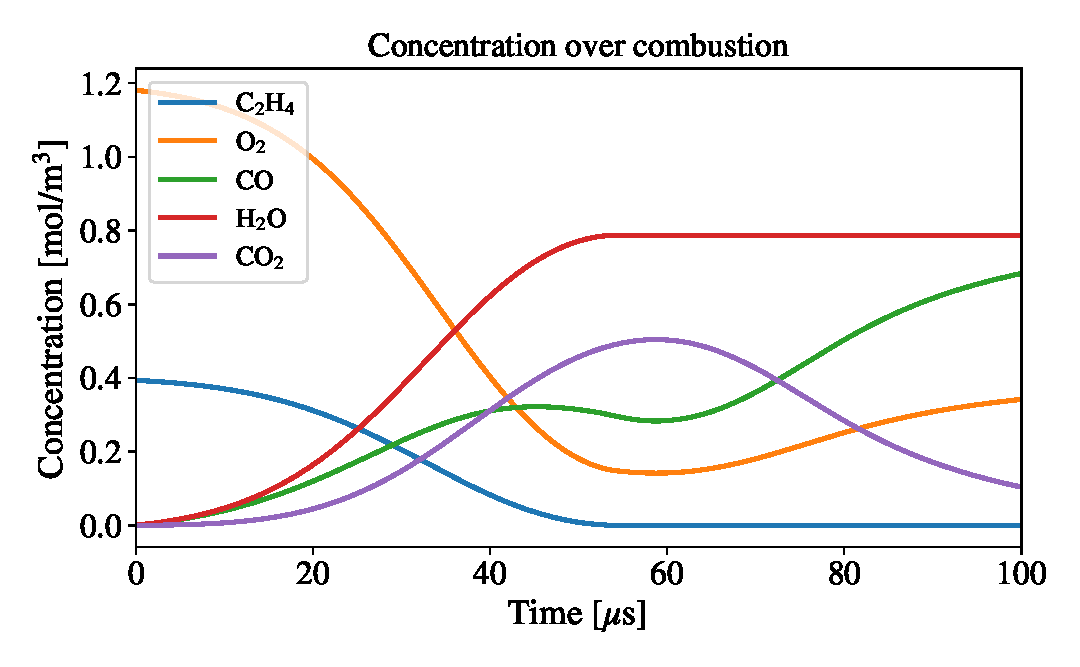
\includegraphics[width=0.9\linewidth]{images/concentration.pdf}
	\caption{Concentration of species over combustion}
	\label{fig:concentration}
\end{figure}

It should be noted that as the solution progressed, it was necessary to clip
values that tended below zero due to machine precision, to prevent complex
valued non-physical solutions from being created. This leads to a discontinuity
in the reaction rate when \ce{C2H4} is fully combusted, which is not noticeable
in the species concentration solution, however can be seen in the rate of heat
release (Fig.~\ref{fig:heatRate}).

\begin{figure}[H]
	\centering
	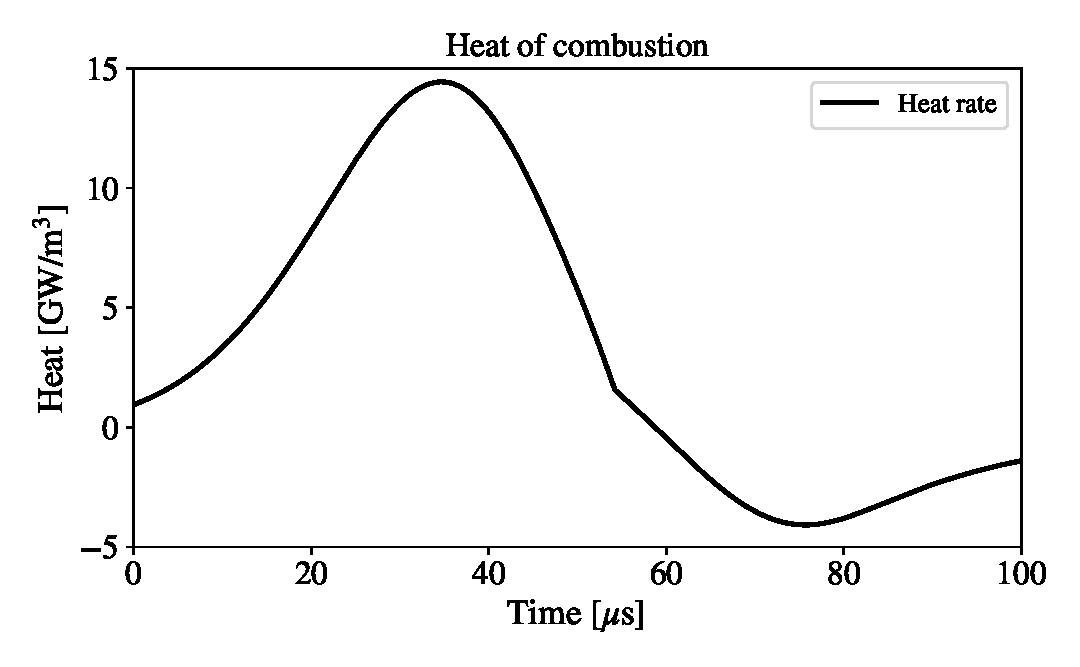
\includegraphics[width=0.9\linewidth]{images/heatRate.pdf}
	\caption{Rate of heat of combustion}
	\label{fig:heatRate}
\end{figure}

\begin{figure}[H]
	\centering
	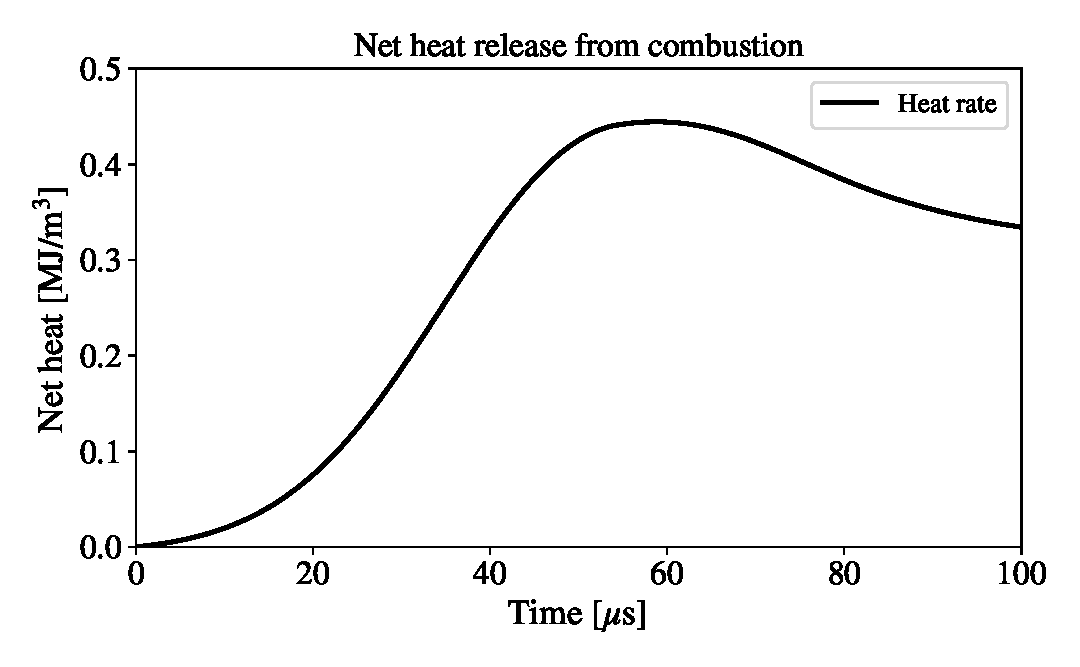
\includegraphics[width=0.9\linewidth]{images/netHeat.pdf}
	\caption{Net heat of combustion}
	\label{fig:netHeat}
\end{figure}

\printbibliography

\newpage
\appendix

\section*{Appendix}

\inputminted[
	tabsize=4,
	obeytabs,
	fontsize=\footnotesize,
	frame=lines,
	framesep=0.5em,
	linenos
]{python}{code/combustionSolver.py}

\end{document}
